\documentclass{eceasst}
% This is an empty ECEASST article that can be used as a template
% by authors.
% Just uncomment the appropriate frontmatter commands and provide
% the parameters.

% Required packages
% =================
% Your \usepackage commands go here.
\usepackage{multirow}
\usepackage{listings}
\usepackage{amsmath}  % for equation*
\usepackage{array}    % for tabular
\usepackage{verbatim} % for comment
\usepackage{wrapfig}
\usepackage[final]{microtype}
\usepackage{tabularx}
\usepackage{mathpartir}
\usepackage{arydshln}

\newcommand\forAll[1]{\forall \, #1 \, . \,}
\newcommand\forAllII[2]{\forall \, #1 \, #2 \, . \,}

\newcommand\propno[1]{(\emph{#1})}
\newcommand\hs[1]{\texttt{#1}}

\newcommand\isaCode[1]{{\fontfamily{lmvtt}\selectfont #1}}
\newcolumntype{?}{!{\vrule width 1pt}}

\lstnewenvironment{code}[1][]
  {\noindent
   \vspace{-0.5\baselineskip}
   \lstset{basicstyle=\ttfamily,
           frame=single,
           language=Haskell,
           keywordstyle=\color{black},
           #1}
   \fontsize{8pt}{8pt}\selectfont}
  {}

% Volume frontmatter
% ==================
% Volume frontmatter for AVoCS 2015
% =====================================
\volume{72}{2015} % Volume number and year
\volumetitle{% Title of the volume (optional)
Proceedings of the\\
15th International Workshop on\\
Automated Verification of Critical Systems
(AVoCS 2015)}
\volumeshort{% Short title of the volume (optional)
Proc.\ AVoCS 2015}
\guesteds{% Multiple guest editors
Gudmund Grov, Andrew Ireland}


% Article frontmatter
% ===================
\title{Conditional Lemma Discovery and Recursion Induction in Hipster} % Title of the article
%\short{} % Short title of the article (optional)
%\author{\autref{1}\sponsor{}} % Authors and references to addresses
\author{Irene Lobo Valbuena and Moa Johansson}
%\institute{\autlabel{1}} % Institutes with labels
\institute{\email{lobo@chalmers.se},  \email{moa.johansson@chalmers.se} \\
Department of Computer Science and Engineering \\Chalmers University of Technology, Gothenburg, Sweden.}

\abstract{
Hipster is a theory exploration tool for the proof assistant Isabelle/HOL.
%
It automatically discovers lemmas about given recursive functions and datatypes and proves them by induction.
%
Previously, only equational properties could be discovered.
%
Conditional lemmas, for example required when reasoning about sorting, has been beyond the scope of theory exploration.
%
In this paper we describe an extension to Hipster to also support discovery and proof of conditional lemmas.

We also present a new automated tactic, which uses \emph{recursion induction}.
%
Recursion induction follows the recursive structure of a function definition through its termination order, as opposed to structural induction, which follows that of the datatype.
%
We find that the addition of recursion induction increases the number of proofs completed automatically, both for conditional and equational statements.
} % Abstract of the article

\keywords{theory exploration, automated induction, interactive theorem proving} % Keywords for the article

\begin{document}
\maketitle

% Main part of your article
% =========================
\section{Introduction}
\label{sec:intro}

Theory exploration is a technique for automatically discovering new interesting lemmas in a formal mathematical theory development.
%
These lemmas are intended to help constructing a richer background theory about the concepts at hand (e.g. functions and datatypes) which can be useful both to enhance the power of automation as well as being of use in interactive proofs \cite{mathsaid,isacosy,isascheme}.
%
Theory exploration has proved particularly useful for automation of inductive proofs \cite{hipspecCADE}. This work builds on Hipster \cite{hipster}, an interactive theory exploration system for the proof assistant Isabelle/HOL \cite{isabelle}.
%
It can be used in two modes, either \emph{exploratory mode} to generate a set of basic lemmas about given datatypes and functions, or in \emph{proof mode}, where it assists the user by searching for missing lemmas needed to prove the current subgoal.
%
To generate conjectures, Hipster uses as a backend the HipSpec system, a theory explorer for Haskell programs \cite{hipspecCADE}.
%
Proofs are then performed by specialised tactics in Isabelle/HOL. Hipster has been shown capable of discovering and proving standard lemmas about recursive functions, thus speeding up theory development in Isabelle.
%
However, lemma discovery by theory exploration has previously been restricted to equational properties.
%
In this paper we take the first steps towards lifting this restriction and exploring also conditional conjectures.
%
Conditional lemmas are necessary if we for example want to prove properties about sorting algorithms.
%
As an example, consider the proof of correctness for insertion sort:
%
%\begin{small}
\begin{center}
\isaCode{theorem isortSorts: "sorted (isort xs)"}
\end{center}
%\end{small}
%
To prove this theorem by induction will in the step-case require a lemma telling us that if a list is sorted, it remains so after an additional element is inserted:
%
\begin{center}		
\isaCode{lemma "sorted xs $\Longrightarrow$ sorted (insert x xs)"}
\end{center}
%
Discovering this kind of conditional lemmas introduces a big challenge for theory exploration.
%
First of all, the search space greatly increases: what statements should be picked as potentially interesting side-conditions to explore?
%
Secondly, as our theory exploration system relies on generation of random test-cases, we also need to ensure that we perform tests where the condition evaluates to true, otherwise we may miss conditional equations as the theory exploration system might place the relevant terms in different equivalence classes (see Example 2 on p. \pageref{example2}).

As Hipster is designed as an interactive system, we avoid the first problem by asking the user to specify under which condition theory exploration should occur.
%
In the example above, this would require the user to tell Hipster that the predicate \isaCode{sorted} is an interesting pre-condition, in addition to which function symbols should be explored in the bodies of lemmas.
%
The rest of the process is however automatic.
%
We describe it in more detail in \S \ref{sec:conditionals} 

The second contribution of this paper is a new automated tactic for \emph{recursion induction} (see e.g. \S3.5.4 of \cite{isabelle}).
%
Previously, Hipster only supported structural induction over the datatypes, but has now been extended with a new tactic that uses recursion induction, following the termination order of function definitions instead of the datatype.
%
This has shown to be useful for many proofs that previously failed, but can also provide shorter proofs in some cases.
%
The new recursion induction tactic is described in \S \ref{sec:rec-ind}.
%
It is used by Hipster during automated theory exploration, but can equally well be applied as a powerful regular tactic by a human user working in Isabelle.


%Background, explaining how Hipster works
\section{Hipster}
\label{sec:background}
This section provides a description of how Hipster works and how its subsystem QuickSpec generates conjectures.

\subsection{Theory Exploration in Hipster}
Figure \ref{fig:hipster} gives an overview of the Hipster system.
%
Starting from an Isabelle theory file that defines a set of datatypes and functions, the user calls Hipster on a list of functions about which she is interested in finding lemmas.
%
The workings of Hipster can be divided up into three stages:
\begin{enumerate}
\item Generation of Haskell code. 
\item Theory exploration in Haskell.
\item Proof in Isabelle.
\end{enumerate}

\begin{figure}[htbp]
\begin{center}
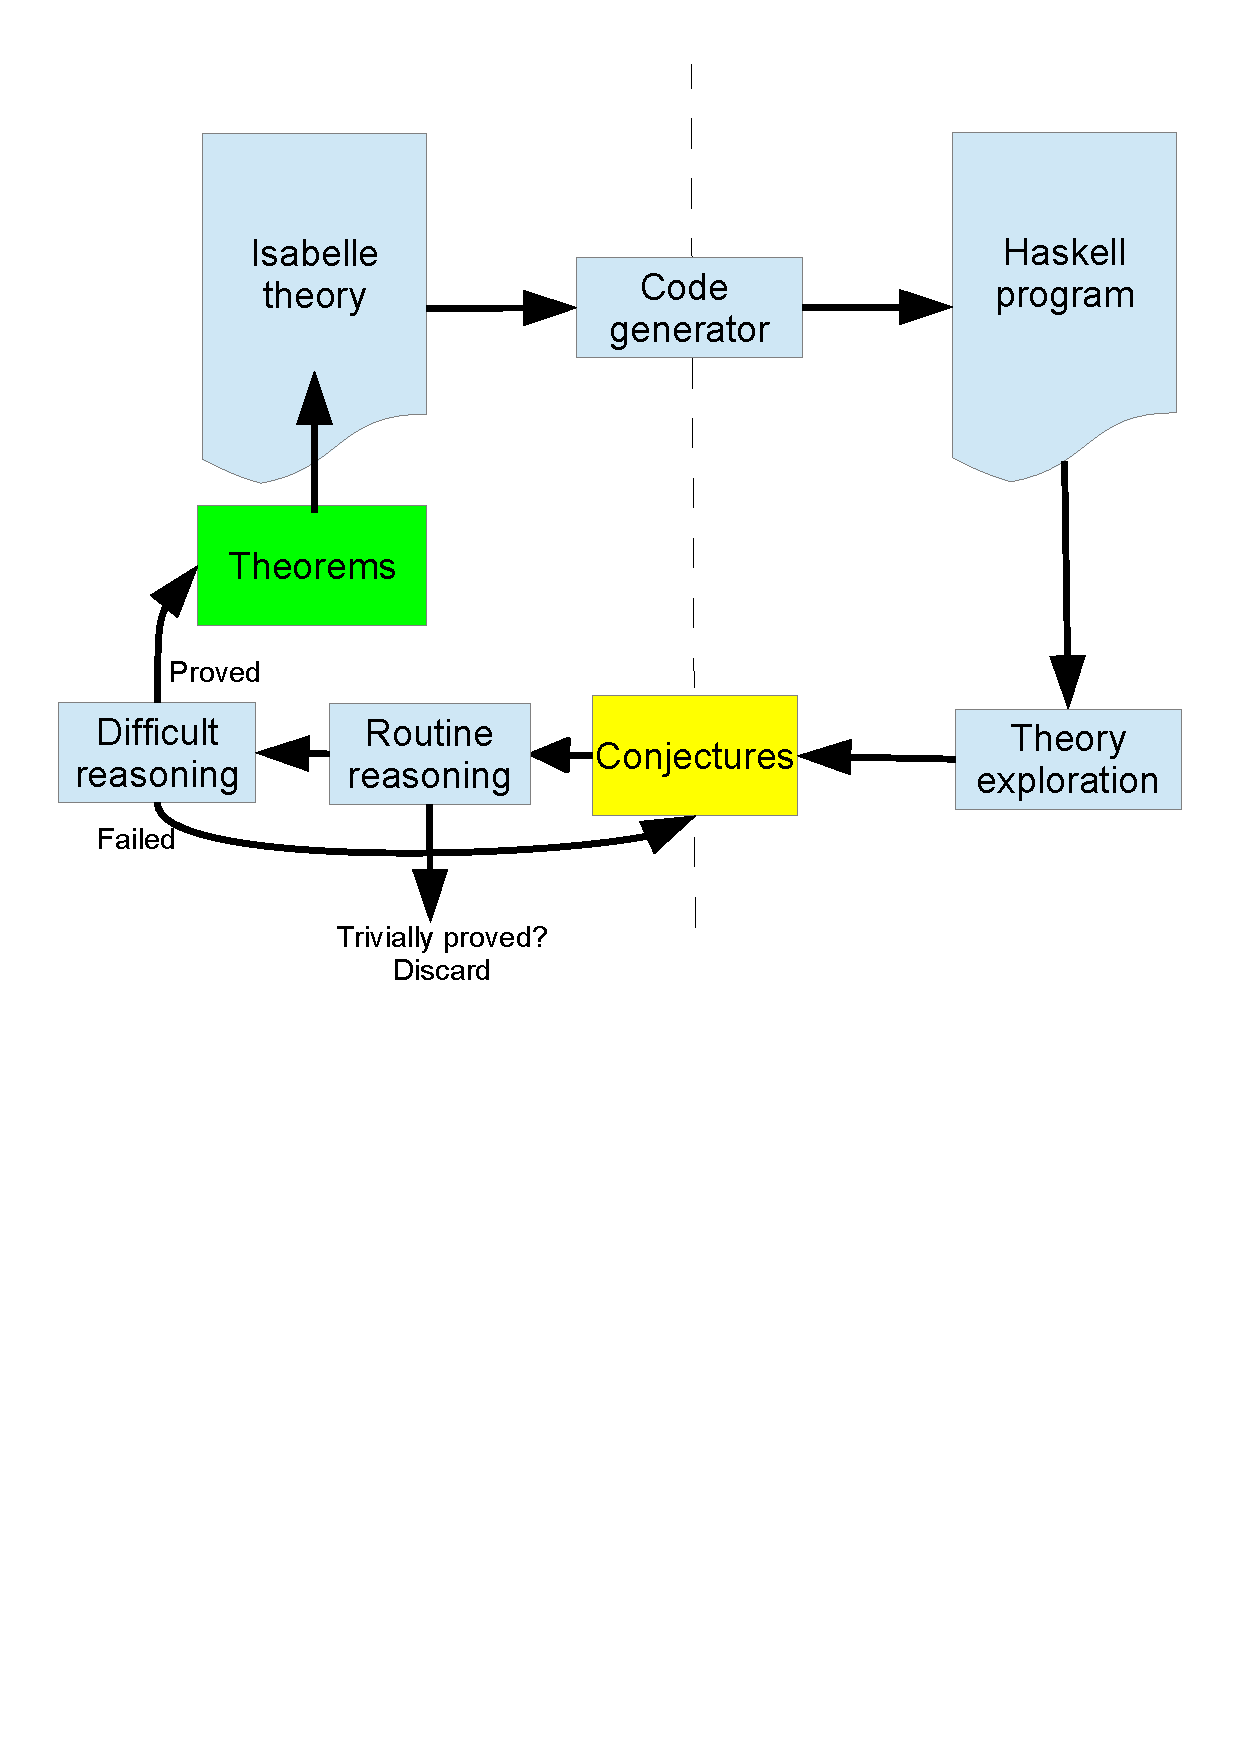
\includegraphics[scale=0.4]{hipster}
\caption{Overview of Hipster}
\label{fig:hipster}
\end{center}
\end{figure}

Hipster uses Isabelle's code generator \cite{codegen2}, to translate the theory to a Haskell program.
%
Hipster then employs the theory exploration system HipSpec as a backend for generating conjectures.
%
While HipSpec can be used also as a fully fledged theorem prover, Hipster only uses its conjecture generation subsystem QuickSpec \cite{quickspec}, and performs proofs inside Isabelle.
%
Isabelle is an LCF-style prover, which means that it is based on a small core of trusted axioms, upon which subsequent proofs must be built.
%
Therefore, any proofs found outside Isabelle, e.g. by HipSpec, would have to be reconstructed inside Isabelle anyway.
%
Hence it is easier for Hipster to simply use Isabelle for proofs in the first place. 

Not all conjectures returned from QuickSpec are interesting.
%
Hipster is parametrised by two tactics, which can be set by the user: one for \emph{routine reasoning} and one for \emph{difficult reasoning}.
%
Conjectures solved by routine reasoning are deemed trivial and discarded, while those requiring more difficult reasoning are displayed to the user and included in the Isabelle theory so they can be used in subsequent proofs if necessary.
%
In the context of this paper, routine reasoning is first-order equational reasoning and simplification, while difficult reasoning involves some kind of induction. If a conjectur is not immediately provable, Hipster will place it at the end of the list of open conjectures and will try it again if it has found some additional lemmas.
%
Occasionally, Hipster might discover some conjecture which it does not manage to prove automatically, because not even its tactic difficult reasoning is strong enough. Such an open conjecture would also be displayed to the user, who can then choose to perform an interactive proof in Isabelle, perhaps employing other tactics or lemmas than those currently available to Hipster.


\subsection{Conjecture Generation in QuickSpec}
% XXX: "by default three per type" ?
QuickSpec takes as input a set of functions and variables (by default three per type), and generates all type-correct terms up to a given limit (by default depth three).
%
The number of variables and term-depth limit can be adjusted by the user.
%
QuickSpec then proceeds to divide the generated terms into equivalence classes, so that each equivalence class eventually represents a set of equations.
%
Initially, all terms of the same type are in the same equivalence class. QuickSpec then uses QuickCheck \cite{quickcheck}, to generate random ground values for the variables in the terms, and evaluates the result.
%
If two terms in an equivalence class turn out to evaluate differently, the equivalence class is split accordingly.
%
The process is then repeated until the equivalence classes stabilise (after several hundred different random tests), which means that we usually have quite a high confidence in that the conjectures produced are probably true, even though they are not yet proved.  

% This paragraph could possibly be in the next section on conditional lemmas, but it feels like it belongs to the Background section in a way...
%The support in QuickSpec for generating conditional conjectures (implications) is still rather basic.
%%
%In this case, QuickSpec will in addition to the other input require the user to specify a predicate to use as the premise of an implication.
%%
%Term generation proceeds as described above, but testing takes the given predicate into account.
%%
%Here, we are only interested in tests with values that make the premise true, otherwise we may split the equivalence classes when they should not be split.
%%
%QuickCheck uses special functions called \emph{generators} to produce random values of a given type.
%%
%If using QuickSpec directly in Haskell, the user can program special purpose generators that could be made to only produce values satisfying a given predicate.
%%
%In Hipster, however, these generator functions are simpler as they have to be automatically derived together with the Haskell code.
%%
%Tests not satisfying the premise are simply discarded during conditional exploration, which means that we typically must generate more tests than for equational conjectures.
%%
%Also, the risk of some non-theorem slipping through is slightly higher, but as Hipster then attempts to prove all conjectures, such a statement would be caught in the proving phase.
%%
%Automatically generating customised generator functions is further work. 

%%% Example if there is space %%%
\paragraph*{Example 1.}
\label{example1}
As a small example, consider a theory exploration attempt where we have asked Hipster for lemmas about a function \isaCode{isort} implementing insertion sort.
%
%We are furthermore interested in the case with the condition that the predicate \isaCode{sorted} holds (for one variable). %Among the terms generated by QuickSpec are for example: \isaCode{xs}, \isaCode{sort xs}, \isaCode{sort(sort xs)}. 
%QuickSpec first performs one pass looking for plain equations, then a second where it considers the condition \isaCode{sorted xs}. 
%
%We start with the first phase, where QuickSpec investigates non-conditional conjectures.
%%
Among the terms generated by QuickSpec are those in the table below.
%
Initially, all terms are placed in the same equivalence class.
%
Suppose QuickSpec generates the random value \isaCode{xs} $\rightarrow$ \isaCode{[3,1]}.     

\vspace{2 mm}

\noindent \begin{tabularx}{\textwidth}{l  X  X  X}
 & Term & Ground Instance & Value \\
 \hline
1 \quad &\isaCode{isort xs} & \isaCode{isort [3,1]} & \isaCode{[1,3]} \\
2 \quad&\isaCode{isort (isort xs)} &\isaCode{isort (isort [3,1])} & \isaCode{[1,3]}\\  
3 \quad &\isaCode{xs} &\isaCode{[3,1]} & \isaCode{[3,1]} \\
\end{tabularx}

\vspace{2 mm}

\noindent As not all terms evaluate to the same value, they should no longer be in the same equivalence class. We thus split the terms into two new equivalence classes: terms 1 and 2 evaluate to the same value and remain together, while term 3 is separate.
%
After this, no subsequent tests further split these equivalence classes, and we can read off the equation: \isaCode{isort(isort xs) = isort xs}.  
%
%In the second phase, QuickSpec performs a new exploration, this time requiring the predicate \isaCode{sorted xs} to hold for all test values.
%%
%Suppose we test with the sorted list: \isaCode{xs $\rightarrow$ [1,2]} (other non-sorted values for \isaCode{xs} would be discarded).       
%
%\vspace{2 mm}
%
%\noindent \begin{tabularx}{\textwidth}{l  X  X  X}
% & Term & Ground Instance & Value \\
% \hline
%1 \quad &\isaCode{sort xs} & \isaCode{sort([1,2])} & \isaCode{[1,2]} \\
%2 \quad &\isaCode{sort (sort xs)} &\isaCode{sort (sort [1,2])} & \isaCode{[1,2]}\\
%3 \quad &\isaCode{xs} &\isaCode{[1,2]} & \isaCode{[1,2]} \\
%\end{tabularx}
%
%\vspace{2 mm}
%
%\noindent This time, all terms evaluate to the same value on all tests where the list is sorted, so all three terms remain in the same equivalence class.
%%
%QuickSpec realises that there is no point producing the conjecture \isaCode{sorted xs $\Longrightarrow$ sort (sort xs) = xs}, as this is subsumed by the non-conditional equation discovered in the first phase.
%%
%It will however produce the additional conjecture \isaCode{sorted xs $\Longrightarrow$ sort xs = xs}, which clearly only holds if the list is already sorted.
%



% Conditional lemmas, with a worked example
\section{Conditional Lemmas and Recursion Induction}
\label{sec:conditionals}

We now demonstrate how to employ Hipster interactively for theory exploration of conditional lemmas in the development of a theory, with the aim of proving insertion sort's correctness.
%
We first explain how conditional conjectures are generated in QuickSpec.
%
We then explain our new automated induction tactic for recursion induction, and finally show how Hipster combines these in a case study proving the correctness of insertion sort.  

\subsection{Generating Conditional Conjectures}
The support in QuickSpec for generating conditional conjectures (implications) is still rather basic.
%
In this case, QuickSpec will in addition to the other input require the user to specify a predicate to use as the premise of an implication.
%
Term generation proceeds as described above, but testing takes the given predicate into account.
%
Here, we are only interested in tests with values that make the premise true, otherwise we may split the equivalence classes when they should not be split.
% newpara?
QuickCheck uses special functions called \emph{generators} to produce random values of a given type.
%
If using QuickSpec directly in Haskell, the user can program special purpose generators that could be made to only produce values satisfying a given predicate.
%
In Hipster, however, these generator functions are simpler as they have to be automatically derived together with the Haskell code.
%
Tests not satisfying the premise are simply discarded during conditional exploration, which means that we typically must generate more tests than for equational conjectures.
%
Also, the risk of some non-theorem slipping through is slightly higher, but as Hipster then attempts to prove all conjectures, such a statement would be caught in the proving phase.
%
Automatically generating customised generator functions is further work. 

\paragraph*{Example 2.}
\label{example2}
In Example 1, we showed how QuickSpec generated equational conjectures about the insertion sort function \isaCode{isort}.
%
We are furthermore interested in the case with the condition that the predicate \isaCode{sorted} holds (for one variable).
%
QuickSpec now first performs one pass looking for plain equations, as in Example 1, then a second where it considers the condition \isaCode{sorted xs}.
%
In the second phase, QuickSpec performs a new exploration, this time requiring the predicate \isaCode{sorted xs} to hold for all test values.
%
Suppose we test with the sorted list: \isaCode{xs $\rightarrow$ [1,2]} (other non-sorted values for \isaCode{xs} would be discarded).       

\vspace{2 mm}

\noindent \begin{tabularx}{\textwidth}{l  X  X  X}
 & Term & Ground Instance & Value \\
 \hline
1 \quad &\isaCode{isort xs} & \isaCode{isort([1,2])} & \isaCode{[1,2]} \\
2 \quad &\isaCode{isort (isort xs)} &\isaCode{isort (isort [1,2])} & \isaCode{[1,2]}\\
3 \quad &\isaCode{xs} &\isaCode{[1,2]} & \isaCode{[1,2]} \\
\end{tabularx}

\vspace{2 mm}

\noindent This time, all terms evaluate to the same value on all tests where the list is sorted, so all three terms remain in the same equivalence class.
%
QuickSpec realises that there is no point producing the conjecture \isaCode{sorted xs $\Longrightarrow$ isort (isort xs) = xs}, as this is subsumed by the non-conditional equation discovered in the first phase.
%
It will however produce the additional conjecture \isaCode{sorted xs $\Longrightarrow$ isort xs = xs}, which clearly only holds if the list is already sorted.


%\subsection{A Need for Conditionals}
%
%Conditional lemmas are required in breaking down reasoning into small units of focus.
%%
%Different scenarios and constructs require or give rise to constrained propositions:
%
%\begin{itemize}\itemsep0mm
%\item branching on conditions determining cases during a proof attempt
%\item proving algorithm correctness, where changes of consecutive steps are to be taken into account
%\item programming invariants
%\begin{itemize}\itemsep1mm
%\item in datatypes, where sometimes these cannot be encoded in the constructors and instead depend of the arrangement of data values conforming an instance and invariant preservation by from functions manipulating the datatype
%\item in functions and algorithms, where auxiliary functions might assume certain conditions on their input to be able to guarantee conditions over the output result.
%\end{itemize}
%\end{itemize}
%
%By employing recursion induction, a proof can be driven and shaped by the structure of its components (types or functions), further explained in \S \ref{sec:rec-ind}.
%%
%This allows to account for the imposition a side-condition may have on variables in an explicit, direct way, whether it is via its own recursion induction scheme or its evaluation on cases isolated by another function's recursion induction.

\subsection{Automating Recursion Induction}
\label{sec:rec-ind}

A recursion induction scheme is derived from a function's recursive definition.
%
Unlike structural induction, the recursion induction scheme corresponds to the originating definition and hence, the cases considered in its simplification rules.

When defining a recursive function over an inductive datatype one might traverse arguments following a different pattern to the strictly structural one (the one arising from a datatype's definition).
%
This pattern could be more specific, or even less so, than following the datatype.

For instance, take the functions on lists \isaCode{sorted} and \isaCode{last}:

\begin{lstlisting}[ mathescape, columns=fullflexible,keepspaces, basicstyle=\fontfamily{lmvtt}\selectfont, ]
fun sorted :: "Nat List $\Rightarrow$ Bool" where
  "sorted [] = True"
| "sorted ([x]) = True"
| "sorted (x1 # (x2 # xs)) = (x1 $\le$ x2 & sorted (x2 # xs))"

fun last :: "'a List $\Rightarrow$ 'a" where
  "last ([x]) = x"
| "last (x # xs) = last xs"
\end{lstlisting}

\noindent From these definitions' structures one can derive a new induction principle.
%
Structural induction on lists considers the base-case \isaCode{[]} (the empty list) and step-case \isaCode{x \# xs} (a list with an element inserted at the front).
%
In the case of \isaCode{sorted}, cases are broken down into more detailed ones by including an additional base-case \isaCode{[x]} (the singleton list) and restricting the step-case to lists with at least two elements \isaCode{x1 \# x2 \# xs}.
%
Meanwhile \isaCode{last} is not defined for the case \isaCode{[]} and hence partially defined, meaning the induction scheme it gives rise to is to be completed with such a case.
%
This, in fact, results in the same recursion induction scheme derived from \isaCode{sorted}:

\vspace{2 mm}

\inferrule [SortedInd]
  {P\;([]) \\ \forall u\;\; P\;([u]) \\ \forall r, \; t, \; ts\;\; (P\;(r \;\#\; ts) \; \Longrightarrow\;P\;(t\;\#\; (r\;\#\; ts)))}
  {\forall x \;\; P\;(x)}

\inferrule [LastInd]
  {\forall u\;\; P\;([u]) \\ \forall r, \; t, \; ts\;\; (P\;(r\;\#\; ts) \; \Longrightarrow\;P\;(t \;\#\; (r\;\#\; ts))) \\ P\;([])}
  {\forall x \;\; P\;(x)}

\vspace{2 mm}

Induction determined by these schemata is called \emph{recursion induction} or \emph{computation induction}.
%
They can isolate sub-units not represented in a datatype's structure as being atomic, such as lists with at least two elements in the scheme for \isaCode{sorted}.
%
Recursion induction hence provides an immediate and more specific structure for reasoning about other recursion patterns where a simple structural induction might fail to set appropriate base and step-cases for the induction to succeed.

Within Isabelle/HOL these schemata are automatically derived and proved as theorems from recursive functions' termination order, and hence guaranteed to be sound \cite{krauss-term}. 


\paragraph*{Example 3: Recursion Induction in a Proof.}

%% Example from presentation on difference

To exemplify the potential difference between recursion and structural induction, let us take the already introduced conditional lemma \isaCode{sorted xs $\Longrightarrow$ sorted (insert x xs)}.
%
Applying structural induction on the list \isaCode{xs} would produce the subgoals:

\begin{lstlisting}[ mathescape, columns=fullflexible,keepspaces, basicstyle=\fontfamily{lmvtt}\selectfont, ]
1. sorted [] $\Longrightarrow$ sorted (insert x [])
2. $\wedge$ a y. (sorted y $\Longrightarrow$ sorted (insert x y)) $\Longrightarrow$ sorted (a # y) $\Longrightarrow$
            sorted (insert x (a # y))
\end{lstlisting}

\noindent Whilst \isaCode{sorted}'s recursion induction scheme would yield:

\begin{lstlisting}[ mathescape, columns=fullflexible,keepspaces, basicstyle=\fontfamily{lmvtt}\selectfont, ]
1. sorted [] $\Longrightarrow$ sorted (insert x [])
2. $\wedge$ u. sorted [u] $\Longrightarrow$ sorted (insert x [u])
3. $\wedge$ r t ts. (sorted (t # ts) $\Longrightarrow$ sorted (insert x (t # ts))) $\Longrightarrow$ sorted (r # t # ts) $\Longrightarrow$
               sorted (insert x (r # t # ts))
\end{lstlisting}

\noindent The latter set of subgoals leads to an immediate proof of the main lemma thanks to its steps mirroring the actual predicate definition, hence having a correspondence with its simplification rules.
%
In contrast, the former, even though it intuitively looks immediate to prove, is not sufficiently generalised nor does it specify any intermediate result on inserting an element on a concrete non-empty list (in our case, the singleton list) which would enable to prove the second subgoal for any arbitrary list.
%
Structural induction is in some way a weaker scheme and additional case-splits or lemmas would be required to close the proof employing it in our example.


\subsubsection*{A New Induction Tactic for Hipster}

%I just realised that we're missing this section. Here, we should explain how your new tactic is implemented (i.e. the tactic hipster-induct-schemes used below in the case study). I.e. how it searches for a proof. Does it first try structural induction, and if that that didn't work, proceed to structural induction. Explain how it chooses which functions induction scheme to try if there are several.

We have implemented a new automated tactic for induction in Isabelle, called \isaCode{hipster\_induct\_schemes}.
%
This tactic searches not only for proofs by structural induction, but may also employ recursion induction when appropriate.
%
It is designed for Hipster to use as its "difficult reasoning" component, but human users may of course also employ this tactic in interactive proofs. 

%This is my understanding of what the tactic does. Irene, might need revising!
% I.e. which are the configuration options for the tactic?
The tactic first tries structural induction using the induction scheme associated with the datatype(s) of variables in the problem.
%
If this fails, the tactic then tries recursion induction, using the induction schemes associated with the functions occurring in the problem.
% TODO: TODO: [MENTION heuristics here! Are there any for which functions induction scheme to try first? Timeouts?].
%
For each attempted induction, the tactic will apply Isabelle's simplifier followed by (if necessary) first-order reasoning using Isabelle's built in first-order prover Metis.
%
An overview of the algorithm is shown in Figure \ref{fig:tactic}.
%
The user can configure the tactic to specify what facts should be passed to the simplifier and to Metis.
%
The default is the simplification rules from the relevant function definitions plus the datatype case distinction rules which are automatically derived by Isabelle.
%
We typically often also want to include lemmas discovered by previous theory exploration.
%
However, if we pass too many facts to Metis, it becomes slower.
%
As further work, we plan to experiment with using Sledgehammer instead \cite{sledgehammer}, which calls powerful external first-order provers and reports back exactly which facts were needed in the proof.
%
Metis can then reconstruct the proof quickly inside Isabelle's trusted kernel.

\begin{figure}
\begin{lstlisting}[   mathescape,   columns=fullflexible,   basicstyle=\fontfamily{lmvtt}\selectfont, ]
TRY
  Structural induction schemes(s)
     THEN simplification + F.O. reasoning
OTHERWISE_TRY
  Recursion induction sceheme(s)
     THEN simplification + F.O. reasoning
\end{lstlisting}		
\caption{Overview of Hipsters new tactic.}	
\label{fig:tactic}
\end{figure}


\paragraph*{Example 4: Simultaneous Induction.}
%The new tactic for Hipster explores the proofs one could attain by recursion inductions derived from functions occurring in the conjecture.
%
%As a side-result, this increases the scope of Hipster's original approach for equational lemmas too.

A notable gain of the new tactic with recursion induction is that of having the capability of performing simultaneous induction, whereas previously only structural inductions on a single variable were performed by Hipster.
%
Simultaneous induction schemata are those inducting over more than one variable at a time, whether those variables are of the same type or not.
%
Such is the case for the list function \isaCode{zip}'s recursion induction scheme, which corresponds to parallel induction on two lists:

\begin{lstlisting}[   mathescape,   columns=fullflexible,   basicstyle=\fontfamily{lmvtt}\selectfont, ]
fun zip :: "'a list $\Rightarrow$ 'b list $\Rightarrow$ ('a $\times$ 'b) list" where
  "zip [] y = []"
| "zip (x # xs) [] = []"
| "zip (x # xs) (y # ys) = (x, y) # (zip xs ys)"
\end{lstlisting}

\vspace{2 mm}

\inferrule [ZipInd]
  {\forall ts\;\; P\;([],\; ts) \\ \forall z,\; rs\;\; P\;(z\;\#\; rs, [])  \\ \forall z,\; y,\; rs,\; ts\;\; (P\;(rs,\;ts) \Longrightarrow\; P\;(z\; \# \; rs,\; y\;\#\; ts))}
  {\forall xs, \; ys \;\; P\;(xs,\; ys)}

\vspace{2 mm}

\noindent This scheme, along with some initial theory exploration, allows theorems like the following to be provable automatically:

\begin{lstlisting}[   mathescape,   columns=fullflexible,   basicstyle=\fontfamily{lmvtt}\selectfont, ]
zip (xs @ ys) zs = (zip xs (take (len xs) zs)) @ (zip ys (drop (len xs) zs))
\end{lstlisting}

\noindent Or even the alternative related conditional lemma to be immediately provable:

\begin{lstlisting}[   mathescape,   columns=fullflexible,   basicstyle=\fontfamily{lmvtt}\selectfont, ]
len xs = len ys $\Longrightarrow$ (zip xs ys) @ (zip zs ws) = zip (xs @ zs) (ys @ ws)
\end{lstlisting}

Neither of these lemmas were provable before, even having done exploration for all the occurring functions in them.
%
Hipster's prior structural induction approach could not capture in a scheme the relation between two variables.
%
In these two cases, \isaCode{zip} traverses its arguments taking steps on both at the same time, a pattern we can only capture with some form of simultaneous induction.
%
Instead of synthesising a series of possible simultaneous induction schemata, recursion induction gives us an immediate choice which is also closer to the problem at hand.


\subsection{Interactive Case Study: Insertion Sort}

We here showcase Hipster's handling of conditional lemmas via the proof of correctness for the theorem \isaCode{sorted (isort ts)}.
%
For it, we assume the less-or-equal operator \isaCode{$\le$} for naturals (and no prior, additional lemmas), and the function definitions:

\begin{lstlisting}[ mathescape, columns=fullflexible,keepspaces, basicstyle=\fontfamily{lmvtt}\selectfont, ]
fun sorted :: "Nat List $\Rightarrow$ Bool" where
  "sorted [] = True"
| "sorted ([x]) = True"
| "sorted (x1 # (x2 # xs)) = (x1 $\le$ x2 & sorted (x2 # xs))"

fun insert :: "Nat $\Rightarrow$ Nat List $\Rightarrow$ Nat List" where
  "insert x [] = [x]"
| "insert x1 (x2 # xs) = (if (x1 $\le$ x2) then x1 # (x2 # xs)	
                                           else x2 # (insert x1 xs))"

fun isort :: "Nat List $\Rightarrow$ Nat List" where
  "isort [] = []"
| "isort (x # xs) = insert x (isort xs)"
\end{lstlisting}

Running exploration from the simpler components is the first step, considering both equational and conditional lemmas, since we have two predicates involved in the definiens of functions in the final theorem.
%
The following command invokes conditional exploration for \isaCode{$\le$}:

\begin{lstlisting}[ mathescape, columns=fullflexible,keepspaces, basicstyle=\fontfamily{lmvtt}\selectfont, ]
hipster_cond $\le$
\end{lstlisting}

\noindent which, along with conditional exploration for its negation, results in $10$ discovered and proven lemmas, $6$ of which are conditionals (we present the vital lemmas towards the final proof) and all require recursion induction:

\begin{lstlisting}[ mathescape, columns=fullflexible,keepspaces, basicstyle=\fontfamily{lmvtt}\selectfont, ]
lemma lemma_ac [thy_expl]: "x $\le$ y $\Longrightarrow$ x $\le$ (S y) = True"
by (hipster_induct_schemes $\le$.simps Nat.exhaust)

lemma lemma_ad [thy_expl]: "y $\le$ x $\Longrightarrow$ (S x) $\le$ y = False"
by (hipster_induct_schemes $\le$.simps Nat.exhaust)
(...)
lemma lemma_ai [thy_expl]: "($\lnot$ (x $\le$ y)) $\Longrightarrow$ x $\le$ Z = False"
by (hipster_induct_schemes $\le$.simps Nat.exhaust)
(...)
\end{lstlisting}

\noindent Hipster automatically generates this output.
%
For each case, the \isaCode{lemma} command makes the statement to be proven and is followed by a tactic application via the \isaCode{by} command, here using Hipster's new tactic \isaCode{hipster\_induct\_schemes}, which employs recursion induction where necessary.
%
To enable the completion of the proof, exploration provides it with the automatically generated Isabelle rules for simplification of function definitions, such as \isaCode{$\le$.simps}, and datatype case distinction rules, such as \isaCode{Nat.exhaust}.

With a new exploration considering the functions about sorting itself and (potentially) taking \isaCode{sorted} as a side-condition for which to discover lemmas, Hipster discovers and proves both the conditional auxiliary lemma required and the goal theorem.
%
Note that the exploration command takes as its first argument the predicate with which to construct side-conditions:

\begin{lstlisting}[ mathescape, columns=fullflexible,keepspaces, basicstyle=\fontfamily{lmvtt}\selectfont, ]
hispter_cond sorted isort insert
(...)
lemma isortInvariant [thy_expl]: "sorted ys $\Longrightarrow$ sorted (insert x ys) = True"
by (hipster_induct_schemes sorted.simps isort.simps insert.simps)
(...)
theorem isortSorts [thy_expl]: "sorted (isort x) = True"
by (hipster_induct_schemes sorted.simps isort.simps insert.simps)
\end{lstlisting}

During this last exploration, other interesting lemmas are discovered, all of which can be now proven automatically by using the sub-lemma about \isaCode{insert}'s invariant \isaCode{isortInvariant}:

\begin{lstlisting}[ mathescape, columns=fullflexible,keepspaces, basicstyle=\fontfamily{lmvtt}\selectfont, ]
lemma isortFixes [thy_expl]: "sorted x $\Longrightarrow$ isort x = x"
by (hipster_induct_schemes sorted.simps isort.simps insert.simps)

lemma insertComm [thy_expl]: "insert x (insert y z) = insert y (insert x z)"
by (hipster_induct_schemes insert.simps)
\end{lstlisting}

Invoking the recursion induction tactic \isaCode{hipster\_induct\_schemes} once proves all of the statements above, simplifying the interaction with the proof assistant.
%
Particularly, the crucial lemma \isaCode{isortInvariant} is proven applying \isaCode{sorted}'s associated induction scheme, highlighting once again the need for support of conditional lemmas in automated inductive proving and the possibilities recursion induction brings towards proof automation.

% XXX: include? IF we mention new options
% Lastly, the benefit of an interactive environment is being able to parameterise the proving methods with adequate options as one works along. This supervised automation can be of great utility to a user during a formal theory development.



% Recursion induction
% Merged with section 3 above.
%\section{Automating Recursion Induction}
%\label{sec:rec-ind}

\subsection{Recursion induction}

When defining a recursive function over an inductive datatype one might traverse arguments following a different pattern to the strictly structural one.
%
This pattern could be more specific, or even less so, than the structural one.

For instance, take the functions on lists \isaCode{sorted} and \isaCode{last}:

\begin{lstlisting}[ mathescape, columns=fullflexible,keepspaces, basicstyle=\fontfamily{lmvtt}\selectfont, ]
fun sorted :: "Nat List $\Rightarrow$ Bool" where
  "sorted [] = True"
| "sorted (_ # []) = True"
| "sorted (r # (t # ts)) = (r $\le$ t & sorted (t # ts))"

fun last :: "'a List $\Rightarrow$ 'a" where
  "last (t # []) = t"
| "last (_ # ts) = last ts"
\end{lstlisting}

\noindent From these definitions' structures one can derive two new induction principles.
%
In the case of \isaCode{sorted}, cases are broken down into more detailed ones whilst \isaCode{last} is partially defined, meaning the induction scheme it gives rise to is to be completed with its missing case for empty lists, as the corresponding induction scheme depicts:

\inferrule [SortedInd]
  {P\;([]) \\ \forall u\;\; P\;(u \;\#\; []) \\ \forall t, \; r, \; ts\;\; ((t\;\#\; r \; \Longrightarrow\; P\;(r \;\#\; ts)) \; \Longrightarrow\;P\;(t\;\#\; (r\;\#\; ts)))}
  {\forall x \;\; P\;(x)}

\inferrule [LastInd]
  {P\;(u \;\#\; []) \\ \forall r, \; t, \; ts\;\; (P\;(r\;\#\; ts) \; \Longrightarrow\;P\;(t \;\#\; (r\;\#\; ts))) \\ P\;([])}
  {\forall x \;\; P\;(x)}

Induction determined by these schemata is called \emph{recursion induction} or \emph{computation induction}.
%
They can isolate sub-units not represented in a datatypes structure as being atomic, such as lists with at least two elements in the scheme for \isaCode{sorted}.
%
Recursion induction hence provides an immediate and more specific structure for reasoning about other recursion patterns where a simple structural induction would fail to set appropriate base cases for the inductive step to succeed.

Particularly, within Isabelle/HOL these schemata are automatically derived as theorems from recursive functions termination order \cite{krauss-term}.
 
 
\subsection{Recursion induction for conditionals}


\subsection{A tactic (not only) for conditionals}

\subsubsection*{Simultaneous induction}

The final tactic for Hipster explores the proofs one could attain by recursion inductions derived from either elements in a side-condition or in the conclusion of the lemma to be proven.
%
As a side-result, this increases the scope of Hipster's original approach for equational lemmas too.

A notable gain, affecting both conditional and equational lemmas, is that of having the capability of performing simultaneous induction.
%
Such is the case for the list function \isaCode{zip}'s recursion induction scheme, which corresponds to parallel induction on lists:

\inferrule [ZipInd]
  {\forall ts\;\; P\;([],\; ts) \\ \forall z,\; rs\;\; P\;(z\;\#\; rs, [])  \\ \forall z,\; y,\; rs,\; ts\;\; (P\;(rs,\;ts) \Longrightarrow\; P\;(z\; \# \; rs,\; y\;\#\; ts))}
  {\forall xs, \; ys \;\; P\;(xs,\; ys)}

\noindent This scheme, along with some initial theory exploration, allows theorems like the following to be provable:

\begin{lstlisting}[   mathescape,   columns=fullflexible,   basicstyle=\fontfamily{lmvtt}\selectfont, ]
zip (xs @ ys) zs = (zip xs (take (len xs) zs)) @ (zip ys (drop (len xs) zs))
\end{lstlisting}

\noindent Or even the alternative similar conditional lemma to be immediately provable:

\begin{lstlisting}[   mathescape,   columns=fullflexible,   basicstyle=\fontfamily{lmvtt}\selectfont, ]
len a = len b $\Longrightarrow$ (zip a b) @ (zip c d) = zip (a @ c) (b @ d)
\end{lstlisting}


\subsubsection*{Flexibilising Hipster}

% Include or not?

% Very brief overview of other aspects more interaction-oriented that improve Hipster





% The experimental results
\section{Evaluation}
\label{sec:evaluation}

In this section we present an evaluation of Hipster's automated tactics, an analysis which had not been performed for Hipster to the same extent priorly.

Keeping in mind evaluation of automated tools for interactive theorem proving necessarily has to consider some degree of interaction, two forms of evaluation have been carried out\footnote{Source code for Hipster, examples presented and benchmarks are available online: \url{https://github.com/moajohansson/IsaHipster}}:

\begin{itemize}
\item case studies on algebraic data types and operations on them; in particular focusing on inductive theories for natural numbers and lists

\item evaluation on problems from TIP (Tons of Inductive Problems) \cite{tip-benchmarks}, a set of benchmarks and challenge problems for inductive theorem provers.
\end{itemize}

From TIP, we evaluate Hipster over two sets of problems employed in previous works on inductive theorem proving: Johansson, Dixon and Bundy's work on case-analysis for rippling \cite{IsaPcase} (we denote it \emph{case-analysis}), and prior work by Ireland and Bundy on employing proof failure to guide lemma discovery and patch inductive proofs \cite{productiveuse} (we denote it \emph{prod-failure}).
%
We now present these results and compare them with other tools' reported results.


\subsection{Method}

To evaluate performance on TIP, each problem is analysed individually, in isolation from others, to assess how far Hipster can go from bare definitions.
%
Theory explorations were only run for those whenever the problem was not provable by the recursion induction tactic directly, i.e. when the problem was missing helping lemmas.
%
Explorations were first performed on the individual functions appearing in the problem definition, jointly with their auxiliary functions.
%
These were followed by explorations on groups of said functions if required, leaving conditional exploration as the last exploration to be run before defining the problem as non-provable by Hipster.

As already specified, conditional lemma discovery is limited to explore a single predicate at a time to define side-conditions.
%
For the present evaluation this has sufficed.

Additionally, to test Hipster's capacity when working on strictly newly defined theories, no assumptions nor properties from theories in Isabelle/HOL were considered during proof search.
%
As an example, natural numbers are not Isabelle/HOL's, but redefined.
%
Hence, predefined notions of orderings and other properties do not play a part in proofs obscuring the results of Hipster's actual work.
%
In this way, we only consider as the base starting point a set of definitional statements, aligning with the purpose of proving based on structure and construction of programs.

\subsection{Results}

The following table summarises statistics on the two sets of the benchmarks run.
%
Columns \emph{EQ} and \emph{COND} do so for problems defined by an equational and a conditional theorem respectively.

\vspace{2 mm}

\noindent \begin{tabularx}{\textwidth}{l | X X | X X}
  & \multicolumn{2}{c|}{Case-analysis} & \multicolumn{2}{c}{Prod-failure} \\
  &  EQ & COND & EQ & COND \\
  \hline
  Total number of benchmarks & 71 & 15 & 38 & 12 \\
  \hline
  Fully automated & 67 & 14 & 29 & 12 \\
  Partially automated & 4 & 0 & 6 & 0 \\
  \hline
  Prior exploration & 33 & 4 & 34 & 4 \\
  Conditional exploration & 6 & 2 & 2 & 3 \\
  \hline
  Recursion induction & 29 & 6 & 1 & 1 \\
  Recursion induction on sub-lemmas & 16 & 1 & 5 & 0 \\
  \hline
  Filter theorems for FO prover & 3 & 0 & 0 & 0 \\ % XXX: remove this since we don't mention these options?
\end{tabularx}

\vspace{2 mm}


\paragraph{Automation}
%
Overall, the rate of fully automated provability on the benchmark set is 90\%, considering fully automating the solving of a problem only with discovered lemmas and Hipster's automated recursion induction.
%
For conditional lemmas in the test set this rate is higher, 96\%.

A number of theorems (problems $52$, $53$, $72$, $74$ from \emph{case-analysis}; and $2$, $4$, $5$, $20$, $22$, $23$ from \emph{prod-failure}) required one of the following two similar lemmas, not automatically proven in a first instance (neither by structural nor recursion induction):

\begin{lstlisting}[ mathescape, columns=fullflexible,keepspaces, basicstyle=\fontfamily{lmvtt}\selectfont, ]
len (x @ y) = len (y @ x)
count z (x @ y) = count z (y @ x)
\end{lstlisting}

\noindent The failure is associated to less general auxiliary lemmas not being discovered. % Discovery possibly because discovery of lemmas limits constructed terms to a certain depth.

These examples seem to indicate that recursion induction may not suffice when a non-commutative operation nested within another has commuting arguments on both sides of an equality.
%
At least not in the absence of smaller related lemmas corresponding to subgoals.
%
This seems reasonable: the structure of the terms at each side of the equality will differ upon induction.

Nonetheless, proofs for the problems associated to these lemmas can be partially automated.
%
When extracted, the open subgoals are provable by Hipster.
%
Alternatively, for both cases, one can observe that the outermost function applied, \isaCode{len} and \isaCode{count} respectively, acts as a relator function between two datatypes.
%
Furthermore, these will in fact act as relator functions between list concatenation \isaCode{@} and addition for natural numbers \isaCode{plus}.
%
Since \isaCode{plus} does not occur in the problems to be proven, it is not added to the exploration directly.
%
Adding \isaCode{plus} interactively, Hipster discovers and proves automatically the lemmas:

\begin{lstlisting}[ mathescape, columns=fullflexible,keepspaces, basicstyle=\fontfamily{lmvtt}\selectfont, ]
len (x @ y) = plus (len x) (len y)
count z (x @ y) = plus (count z x) (count z y)
\end{lstlisting}

\noindent Along with the commutative law for \isaCode{plus}, also discovered and proven automatically, these enable the automation of the two pending proofs without further intervention.
%
And so, the corresponding TIP problems are solved as well.

% TODO: successive inductions!


\paragraph{Theory exploration}

Just over half of the problems required prior lemma discovery, indicating the benefit of theory exploration.
%
Equational lemmas were much more likely than conditionals to need exploration.
%
Equations are unrestricted and can be more general, potentially requiring more steps to assess different case branches.
%
However, the number of conditional problems in these benchmarks is low, and one cannot draw conclusions as to whether exploration becomes less necessary, or not, when a statement to be proven is constrained by a side-condition.% On the other hand, for these benchmarks, conditionals provided constraints that narrow down cases.

A smaller subset of problems were provable with the aid of conditional exploration, namely those involving functions defined in terms of some predicate.

\paragraph{Recursion induction}

Whereas recursion induction was not necessary as often as theory exploration (whether for the main theorem or auxiliary lemmas), its impact is still notable.

Overall, there seems to be a trade-off between using weaker induction schemes (structural induction) and reducing the number and complexity of needed auxiliary lemmas.
%
Structural induction was always attempted first by the tactic, meaning theorems solved via recursion induction (around a third of the benchmarks) would have not been solved otherwise, at least not with the degree of exploration carried out.
 
The results suggest recursion induction can save on exploration time.
%
It provides appropriate induction patterns that avoid the need for sub-lemmas about specific constructor combinations.


\subsection{Comparison}

% Briefly describe others tested against

Other inductive provers have also been evaluated on the test suites we have presented results for, serving as a good point of comparison.
%
The following table collects the number of problems solved by some of these in comparison with Hipster.
%
Plain figures correspond to fully automated solutions to problems and those in parentheses $(x)$ indicate number of successful proofs after some adaptation of settings.
%
In total, \emph{case-analysis} has $85$ problems whilst \emph{prod-failure} has $50$.
%
Additionally, a last theorem was not evaluated in all of the associated works, as brought up in \cite{SPASSInduction}. Results including such a lemma are given with square brackets $[x]$.

\vspace{2 mm}

\noindent \begin{tabularx}{\textwidth}{l | X X X | X X | X | X | X | X X X}
  & \multicolumn{3}{|c|}{Hipster}
  	& \multicolumn{2}{c|}{HipSpec}
  	& \multicolumn{1}{c|}{Zeno}
  	& \multicolumn{1}{c|}{IsaPlanner}
  	& \multicolumn{1}{c|}{CVC4}
  	& \multicolumn{3}{c}{Pirate} \\
  \hline
  Case-analysis & 80 & (84) & [85] & 80 & & 82 & 47 & 80 & 85 & & [86] \\
  Prod-failure & 41 & (47) & & 44 & (47) & 21 & - & 40 & & (47) & \\
\end{tabularx}

\vspace{2 mm}

\noindent The already mentioned HipSpec uses theory exploration, structural induction and external first-order provers to prove properties about functional programs \cite{hipspecCADE}.
%
Zeno is a tool for proving equational inductive properties of Haskell programs \cite{zeno}.
%
Both CVC4's and Pirate's approaches to inductive proving are built on SMT solving, with a top-down approach in conjecture generation \cite{cvc4, SPASSInduction}.
%
IsaPlanner is a proof planning tool for Isabelle based on rippling \cite{isaplanner2, IsaPcase}.

In comparison to other (automated) inductive provers, the new Hipster is the only one (to the best of our knowledge) to employ recursion induction.
%
As results show, its performance is on par to other state of the art tools'.
%
To be noted is that the failing problems for Hipster in the benchmark set \emph{prod-failure} (problems $33$-$35$) differ from those HipSpec and Pirate fail at (with the exception of $33$ in Pirate's case).
%
These three problems involve definitions for multiplication, factorial and exponentiation operations for Peano numerals with accumulator arguments.
%
Particularly, HipSpec employed adjusted settings in these three cases due to memory usage during testing in QuickSpec to be able to discover appropriate helping lemmas.
%
Hipster has not been evaluated with adjusted settings at the HipSpec/QuickSpec level and hence the exploration phase was not feasible to perform for them.
%
With similar settings to HipSpec's, there is a probability problems $33$-$35$ would be solvable in Hipster too.





\section{Related Work}
\label{sec:related}

The work on lemma discovery for inductive proofs has mainly focused on equational lemmas, for instance in the theory exploration systems IsaScheme and IsaCoSy \cite{isascheme,isacosy}, which also works on Isabelle/HOL theories. IsaScheme requires the user to provide \emph{term schemas}, which are then automatically filled in with available symbols. IsaCoSy only generates irreducible terms, and use an internal constraint language to avoid generating anything that could be reduced by a known equation. These systems focused more on automation, while Hipster is designed to be useable in an interactive theory development. Hipster is faster, and now also supports conditional theory exploration where the user specifies an interesting condition. Conditional lemma discovery has also been missing from the IsaPlanner system, which use \emph{proof critics} to deduce lemmas from failed proof attempts \cite{isaplanner2,IsaPcase}. 

Theory exploration systems relies on having an automated prover at hand to prove generated conjectures. In the context of inductive theories, most other automated provers supporting induction such as IsaPlanner, Zeno, HipSpec, Dafny and CVC4 \cite{isaplanner2, zeno, hipspecCADE,dafny,cvc4} only support structural induction. Hipster now also provides an automated tactic for recursion induction by exploiting Isabelle's automated derivation of such induction schemes. It can both be used in theory exploration and as a stand-alone automated tactic. 

The use of recursion induction and the fact that Hipster produce LCF-style re-checkable proofs is also the main difference between Hipster and its sister system HipSpec \cite{hipspecCADE}, with which Hipster shares its conjecture generation component. HipSpec does instead rely on external first-order provers to solve the proof obligations arising in the step- and base-cases for inductive proofs, and does not produce checkable proofs. 

\section{Conclusion and Further Work}
\label{sec:conclusion}

Generation of conditional lemmas in theory exploration is a challenging problem, not least as it is difficult for a tool to automatically assess which side conditions are interesting.
%
Hipster is an interactive theory exploration system, and gets around this obstacle by relying on the user to decide which predicates are deemed interesting as conditions.
%
In this paper we have also presented a new automated tactic for recursion induction, which improves the level of proof automation of discovered conjectures in Hipster.
%
It can also be used as a powerful stand-alone induction tactic in Isabelle. 
%
Further work on the proving side includes experimenting with different heuristics for choosing which function's recursion induction scheme is most likely to produce a proof, as well as extending Hipster with tactics that can handle mutual- and co-induction automatically.
%Identifying which functions to pick for exploration, also from other theories (e.g. . plus and length)

%More efficient conjecture generation forthcoming in a soon to be released version of QuickSpec.
Hipster has various configuration options for adjusting which of the discovered lemmas are passed to its tactics in subsequent proofs.
%
For example, in larger theories, with many explorations, we may not want to pass all discovered lemmas to Isabelle's Metis tactic, as too many lemmas might slow down the proof process.
%
We plan to experiment with combining Hipster's tactics with the relevance filtering ideas used in Sledgehammer \cite{mash}.
%
Another item of further work is to extend Hipster to produce structured proofs in Isabelle's Isar language, instead of just a one-line application of Hipster's custom tactics.
%
This will be easier to read for a human user, and can be more streamlined, not needing to repeat the search done in the automatic proof found by Hipster's powerful tactics. 



% Acknowledgements for colleagues, referees, ...
% ==============================================
%\begin{acknowledge}
%\end{acknowledge}

% Bibliography with BibTeX
% ========================
\bibliographystyle{eceasst}
\bibliography{bibfile}

\end{document}
